\question\label{q:2}%[15]
	Un sistema satelital consta de $n$ componentes y funciona en un día cualquiera si al menos $k$ de los $n$ componentes funcionan ese día. En un día lluvioso, cada uno de los componentes funciona independientemente con probabilidad $p_1$, mientras que en un día seco cada uno funciona independientemente con probabilidad $p_2$. Si la probabilidad de que llueva mañana es de $\alpha$, ¿cual es la probabilidad de que el sistema satelital funcione?

	\begin{solutionorlines}
		Sea $k$ el número de componentes en funcionamiento en un día determinado. Primero, aplique la ley de probabilidad total al condicionar en día lluvioso o día seco:
		\begin{equation*}
		\mathds{P}\left(X\ge k\right)=\mathds{P}\left(X\ge k\mid\textbf{día lluvioso}\right)+\mathds{P}\left(X\ge k\mid\textbf{día seco}\right).
		\end{equation*}
		Ahora tome por ejemplo $\mathds{P}\left(X\ge k\mid \textbf{día lluvioso}\right)$. Esto es,
		\begin{equation*}
		\mathds{P}\left(X\ge k\mid\textbf{día lluvioso}\right)=\mathds{P}\left(X=k\mid\textbf{día lluvioso}\right)+\cdots+\mathds{P}\left(X=n\mid\textbf{día lluvioso}\right),
		\end{equation*}
		donde
		\begin{equation*}
		\mathds{P}\left(X\mid\textbf{día lluvioso}\right)\sim\mathrm{binomial}\left(n,p_1\right).
		\end{equation*}
		De manera similar, para la probabilidad $\mathds{P}\left(X\ge k\mid \textbf{día seco}\right)$. Esto es,
		\begin{equation*}
		\mathds{P}\left(X\ge k\mid\textbf{día seco}\right)=\mathds{P}\left(X=k\mid\textbf{día seco}\right)+\cdots+\mathds{P}\left(X=n\mid\textbf{día seco}\right),
		\end{equation*}
		donde
		\begin{equation*}
		\mathds{P}\left(X\mid\textbf{día seco}\right)\sim\mathrm{binomial}\left(n,p_2\right).
		\end{equation*}
		Además, nos pide calcular $\mathds{P}\left(X\ge k\mid \textbf{llueva mañana} \right)$, esto es, de la definición de probabilidad condicional:
		\begin{align*}
		\mathds{P}\left(X\ge k\mid \textbf{llueva mañana} \right)
		&=\frac{\mathds{P}\left(X\ge k\cap \textbf{llueva mañana} \right)}{\mathds{P}\left(\textbf{llueva mañana} \right)}\\
		&=\frac{\mathds{P}\left(X\ge k\cap \textbf{llueva mañana} \right)}{\alpha}
		\end{align*}

		\begin{align*}
		\intertext{Primero, calculamos}\\
			\mathds{P}\left(X\ge k\mid \textbf{día lluvioso}\right) &=\mathds{P}\left(X= k\mid \textbf{día lluvioso}\right)+\cdots+\mathds{P}\left(X= n\mid \textbf{día lluvioso}\right) \\
			&=b\left(k;n,p_1\right)+\cdots+b\left(n;n,p_1\right) \\
			&=\binom{n}{k}{p_1}^{k}{\left(1-p_1\right)}^{n-k}+\cdots+\binom{n}{n}{p_1}^{n}{\left(1-p_1\right)}^{0}.
		\intertext{Luego, calculamos}\\
			\mathds{P}\left(X\ge k\mid \textbf{día seco}\right) &=\mathds{P}\left(X= k\mid \textbf{día seco}\right)+\cdots+\mathds{P}\left(X= n\mid \textbf{día seco}\right) \\
			&=b\left(k;n,p_2\right)+\cdots+b\left(n;n,p_2\right) \\
			&=\binom{n}{k}{p_2}^{k}{\left(1-p_2\right)}^{n-k}+\cdots+\binom{n}{n}{p_2}^{n}{\left(1-p_2\right)}^{0}.
		\end{align*}
		Sumando las dos expresiones de arriba se tiene:
		\begin{multline*}
		\mathds{P}\left(X\ge k\right) = \binom{n}{k}{p_1}^{k}{\left(1-p_1\right)}^{n-k}+\cdots+\binom{n}{n}{p_1}^{n}{\left(1-p_1\right)}^{0}\\
		 + \binom{n}{k}{p_2}^{k}{\left(1-p_2\right)}^{n-k}+\cdots+\binom{n}{n}{p_2}^{n}{\left(1-p_2\right)}^{0}.
		\end{multline*}
		%B\left(n;k,p_1\right)=\sum_{x=0}^{r}b\left(x;n,p\right)
		%\stackrel{H_0}{\sim}
		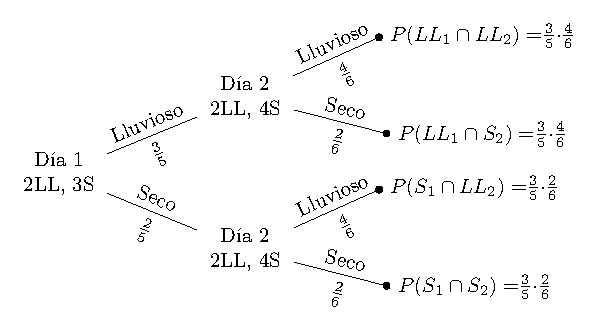
\includegraphics[width=7cm]{fig2}
		\centering
		\captionof{figure}{Diagrama de árbol que ejemplifica la pregunta~\ref{q:2} para algún caso particular.}
		\label{fig:2}
		\justifying
		%Si un equipo de béisbol juega 162 juegos en una temporada y tiene una probabilidad de 50-50 de ganar cualquier juego, entonces la probabilidad de que ese equipo gane más de 100 juegos en una temporada es:
		%https://www.mathworks.com/help/stats/binocdf.html
	\end{solutionorlines}